%% Submissions for peer-review must enable line-numbering
%% using the lineno option in the \documentclass command.
%%
%% Preprints and camera-ready submissions do not need
%% line numbers, and should have this option removed.
%%
%% Please note that the line numbering option requires
%% version 1.1 or newer of the wlpeerj.cls file, and
%% the corresponding author info requires v1.2

\documentclass[fleqn,10pt,lineno]{wlpeerj} % for journal submissions

% ZNK -- Adding headers for pandoc

\setlength{\emergencystretch}{3em}
\providecommand{\tightlist}{
\setlength{\itemsep}{0pt}\setlength{\parskip}{0pt}}
\usepackage{lipsum}
\usepackage[unicode=true]{hyperref}
\usepackage{longtable}



\usepackage{lipsum}

\title{`rstanguts': Bayesian inference of GUTS models with R using Stan
language}

\author[1]{Virgile Baudrot}

\corrauthor[1]{Virgile Baudrot}{\href{mailto:virgile.baudrot@posteo.net}{\nolinkurl{virgile.baudrot@posteo.net}}}
\author[1]{Sandrine Charles}


\affil[1]{UMR CNRS 5558 LBBE, Université Lyon 1, 43 Boulevard du 11 Novembre 1918,
69100 Villeurbanne}


%
% \author[1]{First Author}
% \author[2]{Second Author}
% \affil[1]{Address of first author}
% \affil[2]{Address of second author}
% \corrauthor[1]{First Author}{f.author@email.com}

% 

\begin{abstract}
The toxicokinetic-toxicodynamic (TKTD) modeling approach proved to be of
particular interest in strengthening the Environmental Risk Assessment
(ERA) of chemicals compounds. TKTD models describe the time-course of
processes leading to toxicity at the level of organisms. These models
may include all mechanisms from the toxicokinetics part describing the
compound fate from external concentration to internal kinetics (e.g.,
exposure, uptake, elimination, biotransformation, internal
distribution), and translate the internal concentration into
toxicodynamics covering alteration of cells and organs functioning that
can eventually lead to a toxic effect at the organism level (e.g.,
mortality, reduced reproduction, abnormal behavior) then affecting the
population dynamic. While an integrative mathematical framework as GUTS
offers an efficient theoretical approach, its practical use for
parameter estimation is challenging (from model implementation to
parameter estimation), especially with time-variable exposure. Faced
with this difficulty, Bayesian approach for GUTS models has multiple
advantages as (i) using all data provided by the experiments, (ii)
taking into account the knowledge from experts and/or previous studies,
(iii) being still relevant for complex model with small data set, and
(iv) handling uncertainties by providing distributions of parameter
posteriors. To facilitate the access to Bayesian fitting of GUTS models
based on ordinary differential equations, we implemented GUTS models
within R using the the Stan language dedicated to Bayesian statistics.
In this paper, we compare the result of models implementation
(goodness-of-fit and speedups) and provided some guidelines for using
Bayesian approach in ecotoxicology. For survival analysis of organisms
in response to a chemical stressor, the General Unified Threshold model
of Survival (GUTS) is today recognized as a suitable and powerful TKTD
framework incorporating two complimentary death mechanisms: Stochastic
Death (GUTS-SD) and Individual Tolerance (GUTS-IT), from which a large
range of existing models can be derived.
% Dummy abstract text. Dummy abstract text. Dummy abstract text. Dummy abstract text. Dummy abstract text. Dummy abstract text. Dummy abstract text. Dummy abstract text. Dummy abstract text. Dummy abstract text. Dummy abstract text.
\end{abstract}

\begin{document}

\flushbottom
\maketitle
\thispagestyle{empty}

\section*{Introduction}\label{introduction}
\addcontentsline{toc}{section}{Introduction}

References: (Vehtari, Gelman, and Gabry 2017), (Carpenter et al. 2017)

\section*{Mathematical description of GUTS
models}\label{mathematical-description-of-guts-models}
\addcontentsline{toc}{section}{Mathematical description of GUTS models}

References to look at: (Jager and Ashauer 2018), (Jager et al. 2011),
(Delignette-Muller, Ruiz, and Veber 2017), (Baudrot, Preux, et al. 2018)

\section{\texorpdfstring{Implementation of
`rstanguts'}{Implementation of rstanguts}}\label{implementation-of-rstanguts}

References to look at: (Delignette-Muller, Ruiz, and Veber 2017),
(Baudrot, Preux, et al. 2018), (Baudrot, Charles, et al. 2018)

The implementation was done using the \emph{rstantools} package (Gabry
and Goodrich 2017).

\section{Practical Application
Example}\label{practical-application-example}

The package \texttt{rstanguts} is devoted to the analysis of data from
standard toxicity tests. It provides a simple workflow to calibrate GUTS
models. In this section, we illustrate a typical use of
\texttt{rstanguts} on survival data, which can be followed step-by-step
to analyze new datasets as it is also described in the vignette
\texttt{getting-started}.

In the following example, we use a classical data set of \emph{Gammarus
pulex} exposed to diazinon (Ashauer et al. 2010) as used in the R
package \emph{GUTS} from Albert, Vogel, and Ashauer (2016; Albert and
Vogel 2017). This data set is already in the package, so you can have
access to the data simply by using the \texttt{data()} function.

\section*{Help to write the
manuscript}\label{help-to-write-the-manuscript}
\addcontentsline{toc}{section}{Help to write the manuscript}

\subsection*{\texorpdfstring{Some \LaTeX{}
Examples}{Some  Examples}}\label{some-examples}
\addcontentsline{toc}{subsection}{Some \LaTeX{} Examples}

Use section and subsection commands to organize your document. \LaTeX{}
handles all the formatting and numbering automatically. Use ref and
label commands for cross-references.

\subsection*{Figures and Tables}\label{figures-and-tables}
\addcontentsline{toc}{subsection}{Figures and Tables}

Use the table and tabular commands for basic tables --- see Table
@ref(tab:widgets), for example. You can upload a figure (JPEG, PNG or
PDF) using the project menu. To include it in your document, use the
includegraphics command as in the code for Figure @ref(fig:view) below.

Standard \LaTeX references will work as well (e.g.~Fig. \ref{fig:view}).

\begin{figure}

\includegraphics[width=1\linewidth]{view} \caption{An example image.}\label{fig:view}
\end{figure}

\begin{longtable}[]{@{}lr@{}}
\caption{(\#tab:widgets) An Example Table.}\tabularnewline
\toprule
Item & Quantity\tabularnewline
\midrule
\endfirsthead
\toprule
Item & Quantity\tabularnewline
\midrule
\endhead
Widgets & 42\tabularnewline
Gadgets & 13\tabularnewline
\bottomrule
\end{longtable}

\subsection*{Mathematics}\label{mathematics}
\addcontentsline{toc}{subsection}{Mathematics}

\LaTeX{} is great at typesetting mathematics. Let
\(X_1, X_2, \ldots, X_n\) be a sequence of independent and identically
distributed random variables with \(\text{E}[X_i] = \mu\) and
\(\text{Var}[X_i] = \sigma^2 < \infty\), and let
\[S_n = \frac{X_1 + X_2 + \cdots + X_n}{n}
      = \frac{1}{n}\sum_{i}^{n} X_i\] denote their mean. Then as \(n\)
approaches infinity, the random variables \(\sqrt{n}(S_n - \mu)\)
converge in distribution to a normal \(\mathcal{N}(0, \sigma^2)\).

\subsection*{Lists}\label{lists}
\addcontentsline{toc}{subsection}{Lists}

You can make lists with automatic numbering \dots

\begin{enumerate}
\def\labelenumi{\arabic{enumi}.}
\tightlist
\item
  Like this,
\item
  and like this.
\end{enumerate}

or bullet points\ldots{}

\begin{itemize}
\tightlist
\item
  Like this,
\item
  and like this.
\end{itemize}

or with descriptions\ldots{}

\begin{itemize}
\tightlist
\item
  \textbf{Word} Definition
\item
  \textbf{Concept} Explanation
\item
  \textbf{Idea} Text
\end{itemize}

We hope you find write\LaTeX~useful for your PeerJ submission, and
please let us know if you have any feedback. Further examples with dummy
text are included in the following pages.

\section*{Methods}\label{methods}
\addcontentsline{toc}{section}{Methods}

\lipsum[4] 

\begin{equation}
\cos^3 \theta =\frac{1}{4}\cos\theta+\frac{3}{4}\cos 3\theta
\label{eq:refname2}
\end{equation}

\lipsum[5] 

\subsection*{Subsection}\label{subsection}
\addcontentsline{toc}{subsection}{Subsection}

\lipsum[6] 

\paragraph{Paragraph}

\lipsum[7]  \paragraph{Paragraph} \lipsum[8] 

\subsection*{Subsection}\label{subsection-1}
\addcontentsline{toc}{subsection}{Subsection}

\lipsum[9] 

\begin{figure}
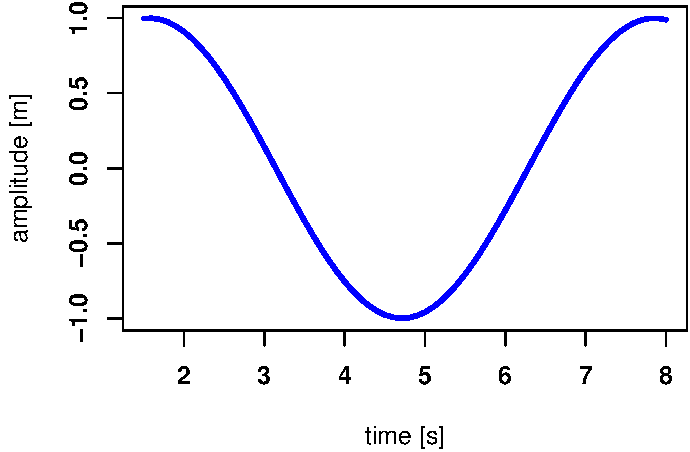
\includegraphics[width=1\linewidth]{manuscript_files/figure-latex/results-1} \caption{In-text Picture}\label{fig:results}
\end{figure}

Reference to Figure @ref(fig:results).

\section*{Results and Discussion}\label{results-and-discussion}
\addcontentsline{toc}{section}{Results and Discussion}

\lipsum[10] 

\subsection*{Subsection}\label{subsection-2}
\addcontentsline{toc}{subsection}{Subsection}

\lipsum[11] 

\subsubsection*{Subsubsection}\label{subsubsection}
\addcontentsline{toc}{subsubsection}{Subsubsection}

\lipsum[12] 

\subsubsection*{Subsubsection}\label{subsubsection-1}
\addcontentsline{toc}{subsubsection}{Subsubsection}

\lipsum[14] 

\subsection*{Subsection}\label{subsection-3}
\addcontentsline{toc}{subsection}{Subsection}

\lipsum[15-20] 

\section*{Acknowledgments}\label{acknowledgments}
\addcontentsline{toc}{section}{Acknowledgments}

So long and thanks for all the fish.

\section*{References}\label{references}
\addcontentsline{toc}{section}{References}

\hypertarget{refs}{}
\hypertarget{ref-Albert2017GUTS}{}
Albert, Carlo, and Sören Vogel. 2017. \emph{GUTS: Fast Calculation of
the Likelihood of a Stochastic Survival Model}.
\url{https://CRAN.R-project.org/package=GUTS}.

\hypertarget{ref-Albert2016}{}
Albert, Carlo, Sören Vogel, and Roman Ashauer. 2016. ``Computationally
Efficient Implementation of a Novel Algorithm for the General Unified
Threshold Model of Survival (Guts).'' \emph{PLoS Comput Biol} 12 (6).
Public Library of Science: e1004978.

\hypertarget{ref-Ashauer2010}{}
Ashauer, Roman, Anita Hintermeister, Ivo Caravatti, Andreas Kretschmann,
and Beate I Escher. 2010. ``Toxicokinetic and Toxicodynamic Modeling
Explains Carry-over Toxicity from Exposure to Diazinon by Slow Organism
Recovery.'' \emph{Environmental Science \& Technology} 44 (10). ACS
Publications: 3963--71.

\hypertarget{ref-Baudrot2018morse}{}
Baudrot, Virgile, Sandrine Charles, Marie Laure Delignette-Muller,
Wandrille Duchemin, Guillaume Kon-Kam-king, Christelle Lopes, Philippe
Ruiz, and Philippe Veber. 2018. \emph{Morse: MOdelling Tools for
Reproduction and Survival Data in Ecotoxicology}.
\url{https://cran.r-project.org/web/packages/morse/index.html}.

\hypertarget{ref-Baudrot2018EST}{}
Baudrot, Virgile, Sara Preux, Virginie Ducrot, Alain Pavé, and Sandrine
Charles. 2018. ``New Insights to Compare and Choose Tktd Models for
Survival Based on an Inter-Laboratory Study for \emph{Lymnaea Stagnalis}
Exposed to Cd.'' \emph{Environmental Science \& Technology}, no. 52, 3
(January). ACS Publications: 1582--90.
doi:\href{https://doi.org/10.1021/acs.est.7b05464}{10.1021/acs.est.7b05464}.

\hypertarget{ref-Carpenter2017stan}{}
Carpenter, Bob, Andrew Gelman, Matthew D Hoffman, Daniel Lee, Ben
Goodrich, Michael Betancourt, Marcus Brubaker, Jiqiang Guo, Peter Li,
and Allen Riddell. 2017. ``Stan: A Probabilistic Programming Language.''
\emph{Journal of Statistical Software} 76 (1). Columbia Univ., New York,
NY (United States); Harvard Univ., Cambridge, MA (United States).

\hypertarget{ref-Delignette-Muller2017}{}
Delignette-Muller, Marie Laure, Philippe Ruiz, and Philippe Veber. 2017.
``Robust Fit of Toxicokinetic--Toxicodynamic Models Using Prior
Knowledge Contained in the Design of Survival Toxicity Tests.''
\emph{Environmental Science \& Technology} 51 (7). ACS Publications:
4038--45.

\hypertarget{ref-Gabry2017rstantools}{}
Gabry, Jonah, and Ben Goodrich. 2017. \emph{Rstantools: Tools for
Developing R Packages Interfacing with 'Stan'}.
\url{https://CRAN.R-project.org/package=rstantools}.

\hypertarget{ref-Jager2011}{}
Jager, Tjalling, Carlo Albert, Thomas G Preuss, and Roman Ashauer. 2011.
``General Unified Threshold Model of Survival - a
Toxicokinetic-Toxicodynamic Framework for Ecotoxicology.''
\emph{Environmental Science \& Technology} 45 (7). ACS Publications:
2529--40.

\hypertarget{ref-Jager2018GUTSbook}{}
Jager, Tjalling, and Roman Ashauer. 2018. \emph{Modelling Survival Under
Chemical Stress. a Comprehensive Guide to the Guts Framework. Version
1.0.} Edited by Leanpud.

\hypertarget{ref-Vehtari2017}{}
Vehtari, Aki, Andrew Gelman, and Jonah Gabry. 2017. ``Practical Bayesian
Model Evaluation Using Leave-One-Out Cross-Validation and Waic.''
\emph{Statistics and Computing} 27 (5). Springer: 1413--32.



\end{document}
